
\chapter{Applied devices}

\section{Robot}

	Define Antropomorf robot
		Mi is ez pontosan, miben különbözik az általános manipulátor robottól
		
		1 kép link a manipulátor robotokról (képként beillesztem majd én -> Patrik)
		
		1 kép link az Antropomorf robotokról (képként beillesztem majd én -> Patrik)

	\subsection{Arduino IDE}
	
		\hspace{15pt}We used Version 1.0.6 of the Arduino IDE to program the Arbotix-M microcontroller. The Arduino IDE is an open-source software which can be used to implement, compile and upload our codes to the microcontroller. The IDE can run on Linux and Mac OS as well as on Windows. Everyone can use the IDE to program any Arduino or Arduino based microcontroller like the Arbotix-M. The environment was created in Java and with other open-source and free software.
	
			\begin{figure}[ht]
				\centering
				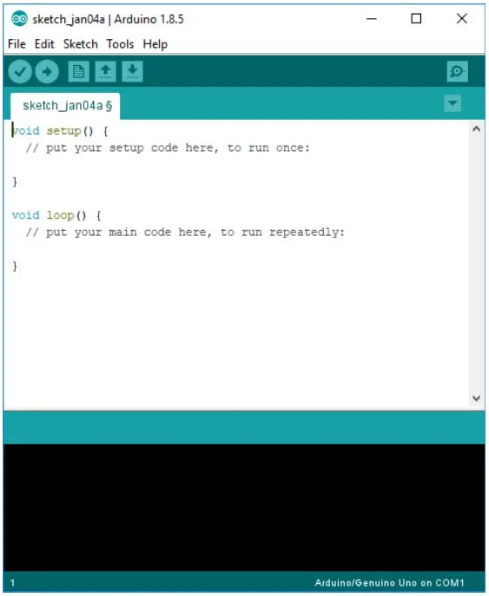
\includegraphics[scale=0.65]{./images/arduino_ide}
				\caption{Arduino IDE \cite{arduino_ide}}
			\end{figure}
			
			\newpage
		
	\subsection{Arbotix-m Robocontroller}
	
		Arduino speciális controllere
		
		Miért is jó ez?

	\subsection{Servo motor}
	
		TODO define milyen Servo motor pontosan -> Dominik
	
		Kép a motorokról + specifikáció link (táblázatként beillesztem majd én -> Patrik)

	\subsection{Equipment}
	e.g.: pincher
	
		Pincher specifikáció (TODO define milyen eszköz pontosa -> Dominik)

\section{Programming language}

miért ez lett?

Arduino környezet jó mert mindent megad 

Stb bullshit